\documentclass[a4paper]{article}

%% Language and font encodings
\usepackage[french]{babel}
\usepackage[utf8x]{inputenc}
\usepackage[T1]{fontenc}

%% Sets page size and margins
\usepackage[a4paper,top=3cm,bottom=3cm,left=2cm,right=2cm,marginparwidth=2cm]{geometry}
%% Useful packages
\usepackage{amsmath}
\usepackage{graphicx}
\usepackage[colorinlistoftodos]{todonotes}
\usepackage[colorlinks=true, allcolors=black]{hyperref}
\usepackage{fourier-orns}
\usepackage{titlesec}
\usepackage{fancyhdr}
\usepackage{fancyvrb}
\usepackage{float}
\pagestyle{fancy} 
\setcounter{tocdepth}{5}



%% Tikz stuff
\usepackage{tikz}
\usetikzlibrary{calc, arrows}
\tikzstyle{incolore} = [rectangle, rounded corners, draw=black, minimum height=1cm, minimum width=3cm, text width=3cm, text centered]



\usepackage{libertine}
\newcommand{\hsp}{\hspace{20pt}}
\newcommand{\HRule}{\rule{\linewidth}{0.5mm}}





\renewcommand{\headrulewidth}{1pt}
\fancyhead[C]{} 
\fancyhead[L]{}
\fancyhead[R]{\footnotesize{\leftmark}}

\renewcommand{\footrulewidth}{1pt}
\fancyfoot[C]{} 
\fancyhead[L]{}
\fancyfoot[R]{\thepage}

\definecolor{Zgris}{rgb}{0.87,0.85,0.85}

\usepackage{eso-pic,graphicx}
\usepackage{xcolor}
\newcommand{\bgimg}[1]{
\AddToShipoutPicture
   {
      \put(\LenToUnit{0 cm},\LenToUnit{0 cm})
      {
            \includegraphics[width=\paperwidth,height=\paperheight]{#1} 
      }
   }
}
\begin{document}




%%\bgimg{Image_15.jpg}

















\begin{titlepage}
    \begin{sffamily}
        \begin{center}
            
\includegraphics[width=5cm]{images/LogoHenallux.PNG}~\\[1.5cm]
            \textsc{\Large Rapport de laboratoire}\\[1.5cm]

            % Title
            \HRule \\[0.4cm]
            { \huge \bfseries Quatrième laboratoire : Fibroptonic\\[0.4cm] }
            \HRule \\[2cm]

            % Author and supervisor
            \begin{minipage}{0.4\textwidth}
                \begin{flushleft} \large
                    Roumache Grégoire\\
                    Sénéchal Julien\\
                    Robert Alexandre\\
                    Wallemme Maxime\\
                    Kenmeugne Lionel\\
                    Didion Charles
                \end{flushleft}
            \end{minipage}
            \begin{minipage}{0.55\textwidth}
                \begin{flushright} \large
                    Laboratoire de sciences appliquées à l'informatique\\
                    Sécurité des systèmes, technologie de l'informatique\\
                    Hénallux\\
                    Première année, groupe H \\
                    Année académique 2019-2020\\
                \end{flushright}
            \end{minipage}
            \vfill

            % Bottom of the page
            {\large 19 Mars 2020}
        \end{center}
    \end{sffamily}
\end{titlepage}







\let\cleardoublepage\clearpage















\section{Introduction}





Pour ce quatrième laboratoire, à cause de la quarantaine, nous avons dû réfléchir, rechercher et analyser les manipulations sans pouvoir les réaliser pour de vrai en laboratoire. Ce travail a donc été difficile à réaliser mais nous espérons que notre travail reste satisfaisant. Nous avons divisé la section \textit{manipulation pratique et analyse} en 6 parties, une pour chaque expérience.















% \section{Rappels théoriques}















\section{Manipulation pratique et analyse}





Dans ce laboratoire, nous avons dû étudier 6 expériences qui sont numérotées 1, 2, 5, 6, 7 et 8 dans le manuel qui sert d'énoncé. C'est pourquoi les numéros des expériences ne se suivent pas.










\subsection{Expérience n\textdegree1 : propagation d’un signal infrarouge dans l’air}





Le but de cette expérience est de montrer que les ondes électromagnétiques infrarouges se propagent dans l’air et dans le verre. On utilise dans cette expérience seulement un photoémetteur et un photorécepteur. Les spectres qu’ils peuvent émettre et réceptionner sont illustré sur la figure \ref{fig:spectresAppareils}.

\begin{figure}[H]
    \centering
    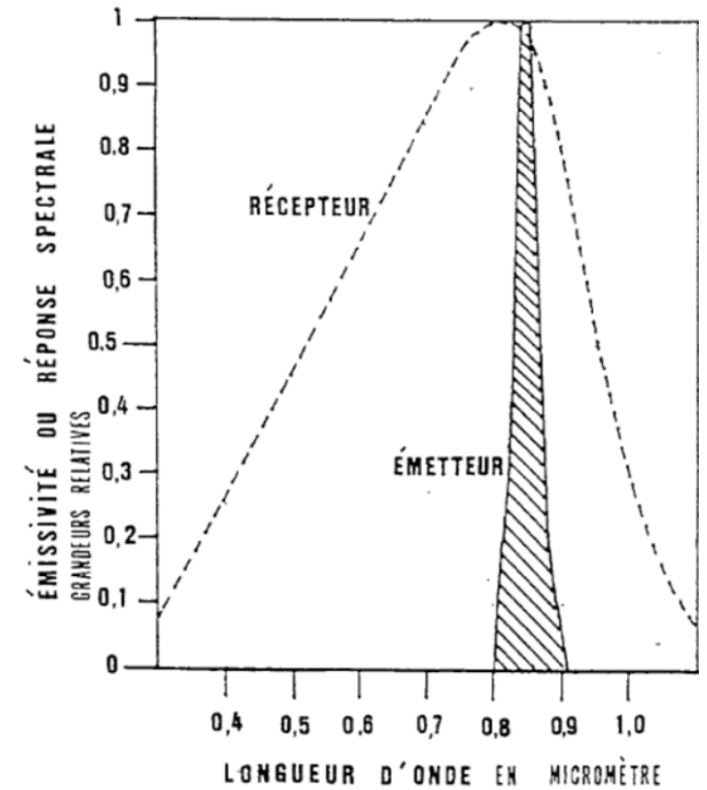
\includegraphics[width=0.65\textwidth]{images/spectres-appareils.PNG}
    \caption{Spectres des ondes lumineuses captées et émises par les appareils}
    \label{fig:spectresAppareils}
\end{figure}

Pour vérifier que la propagation du signal infrarouge dans l’air se fait bel et bien, on va allumer le récepteur sans allumer l’émetteur. La LED rouge du récepteur doit être éteinte car le récepteur ne reçoit évidemment pas de signal. Ensuite, on va allumer l’émetteur, le placer en face du récepteur comme sur la figure \ref{fig:montage01} et vérifier que la LED rouge s’allume, ce qui prouve que le signal infrarouge passe bien dans l’air.

\begin{figure}[H]
    \centering
    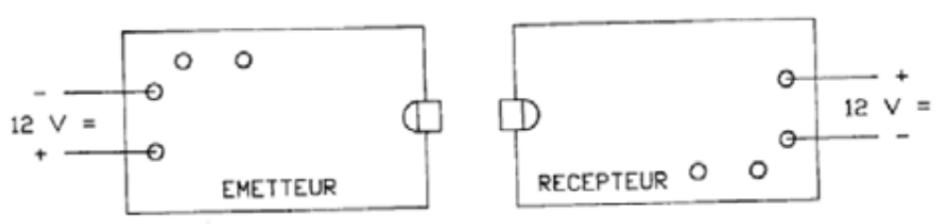
\includegraphics[width=0.95\textwidth]{images/montage01.PNG}
    \caption{Montage de l'expérience n\textdegree1}
    \label{fig:montage01}
\end{figure}










\subsection{Expérience n\textdegree2 : propagation rectiligne d’un faisceau infrarouge}





Cette expérience va nous permettre d'étudier quel est la direction qu'emprunte un faisceau infrarouge et connaître ses propriétés optiques.

Voici tout d'abord, sur la figure \ref{fig:montageExp2} le montage utilisé pour notre expérience.

\begin{figure}[H]
    \centering
    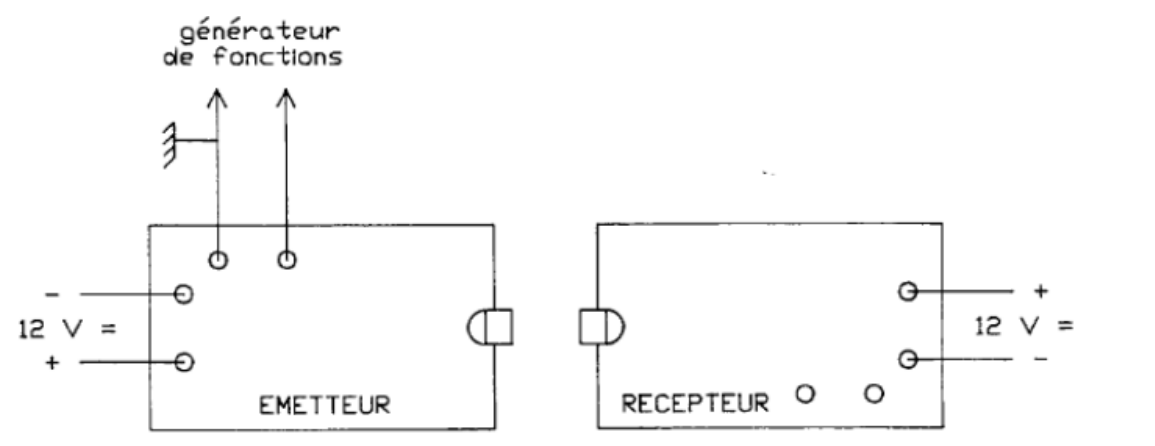
\includegraphics[width=0.95\textwidth]{images/Capture.PNG}
    \caption{Montage de l'expérience n\textdegree2}
    \label{fig:montageExp2}
\end{figure}

\begin{center}
    Signal electrique $\rightarrow$ Emetteur $\Rightarrow$ Signal infrarouge

    Récepteur $\rightarrow$ Haut parleur $\Rightarrow$ Signal acoustique\\[0.4cm]
\end{center}

\emph{"Après avoir réglé le potentiomètre du boîtier récepteur au gain maximal,
on essaie d'aligner le photorécepteur et le photoémetteur."}\\
Un signal sonore retentirat alors même si leur écart en de 10 à 15 cm.\\
\emph{"Par contre, la DEL rouge ne s'allume que pour des distances inférieures à 20 mm"}\\[0.4cm]
Que pouvons donc en conclure :

\begin{enumerate}
    \item On peut voir que l'infrarouge garde une grande directivitée, et donc qu'il garde une trajectoire droite car l'emetteur et le récepteur doivent être exactement face à face si nous voulons que le signal puisse passer.
    \item Le signal électrique a été transformé dans l'emetteur en signal infrarouge.
    \item A l'inverse, dans le recepteur, le signal infrarouge est redevenu un signal acoustique.
\end{enumerate}










\subsection{Expérience n\textdegree5 : propagation d'un signal électromagnétique dans une fibre optique}





Cette manipulation démontre que la fibre optique ne transmet pas   uniquement que des signaux infrarouges. Dans un premier temps j'ai fait des recherche pour me renseigner sur ce qu’est concrètement la fibre et comment elle fonctionne\footnote{\texttt{https://www.youtube.com/watch?v=BIhSb6YMQug}}.

\begin{figure}[H]
    \centering
    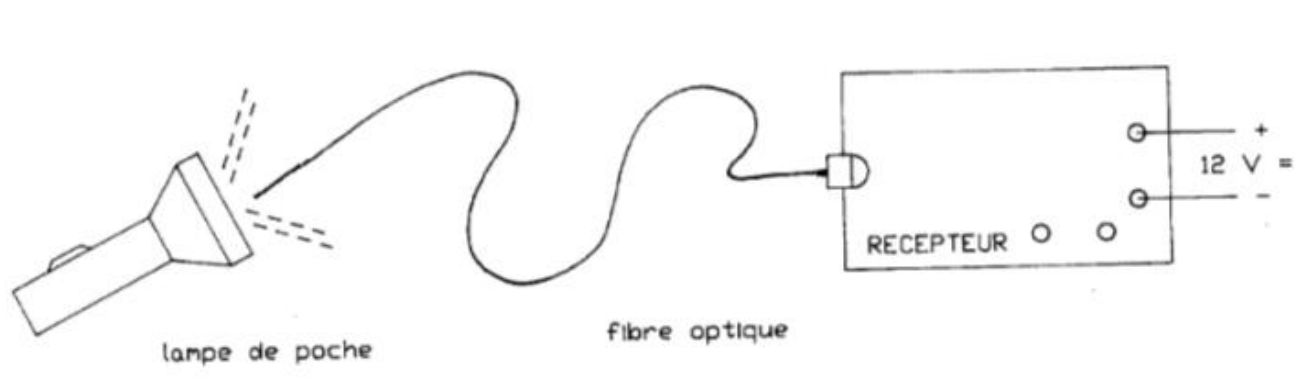
\includegraphics[width=0.95\textwidth]{images/montage02.PNG}
    \caption{Montage de l'expérience n\textdegree5}
    \label{fig:montage02}
\end{figure}

Cette expérience, illustrée sur la figure \ref{fig:montage02}, démontre bien la théorie puisqu’elle prouve que la fibre optique transmet via le cœur du câble un signal lumineux qui n’est pas un signal infrarouge. La lumière émise par la lampe sur le câble a été transmise jusqu'au récepteur et détectée par celui-ci (la lumière se déplaçant en ligne droite).

À noter qu’une grande partie de la lumière émise par la lampe est perdue car seul la partie centrale de la fibre (le cœur) capte la lumière émise toute la couche supérieure plus épaisse qu’on appelle gaine qui, quant à elle, ne capte pas le signal.

Est-elle pour autant inutile ? Outre le fait qu’elle protège le cœur, elle a également pour effet de réguler l’information lumineuse. Elle permet de réfléchir un maximum la lumière soumise au passage à travers un milieu différent (cf. rayon incident $ \rightarrow $ rayon réfracté, réfléchis) pour avoir un signal net qu’on qualifiera de "canalisé".










\subsection{Expérience n\textdegree6 : transmission optique d’une information logique}





Dans cette manipulation, une fibre optique est placée entre un émetteur et un récepteur eux même reliés à un oscilloscope. La DEL verte est alors allumée, et lorsque je place la fibre optique entre les deux, la DEL rouge s’allume car un signal infrarouge est transmis par la fibre optique. Il s’agit de deux états de logique binaire, état 1 le DEL est allumée, état 0 la DEL est éteinte.

Tout cela peut être visualisé sur l’oscilloscope comme montré sur la figure \ref{fig:montage03}.

\begin{figure}[H]
    \centering
    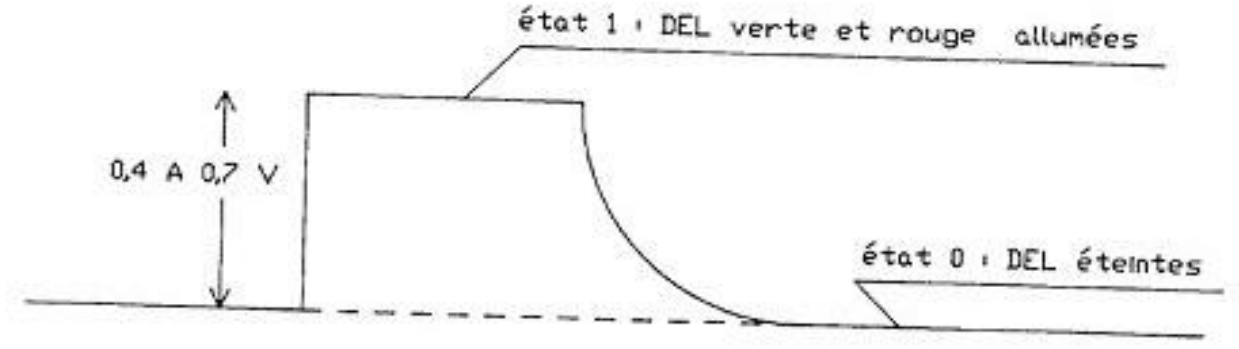
\includegraphics[width=0.95\textwidth]{images/montage03.PNG}
    \caption{Oscillogramme}
    \label{fig:montage03}
\end{figure}

Lorsque le signal infrarouge est transmis par la fibre optique, on observe une montée du signal de 0.4 à 0.7 V montrant ainsi l’état 1. Lorsque le signal n’est plus transmis, on observe une baisse de celui-ci menant donc à l’état 0. On peut donc voir que lorsqu’il y a une montée du signal, cela correspond bien à un signal binaire qui se situe normalement soit à 1, soit à 0 (haut ou bas).










\subsection{Expérience n\textdegree7 : téléphonie par fibre optique}





\begin{figure}[H]
    \centering
    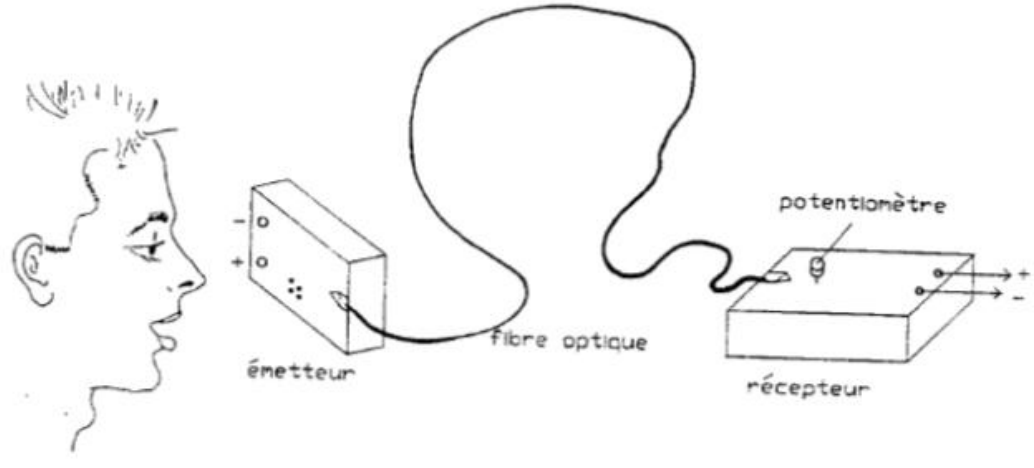
\includegraphics[width=0.85\textwidth]{images/montage05.PNG}
    \caption{Montage de l'expérience n\textdegree7}
    \label{fig:montage05}
\end{figure}

Dans cette manipulation, illustrée par la figure \ref{fig:montage05}, on cherche à montrer qu'on peut moduler le signal sonore au niveau de l'émetteur, l'envoyer sous forme de signal électromagnétique infrarouge dans la fibre optique et le reconstituer au niveau du récepteur.

On peut aussi utiliser un oscilloscope et le connecter au récepteur afin d'illustrer le signal avec un oscillogramme.










\subsection{Expérience n\textdegree8 : transmission optique d’un signal électrique, par fibre optique}





Le but de cette manipulation est d’illustrer la transmission d’un signal électrique par fibre optique.

\begin{figure}[H]
    \centering
    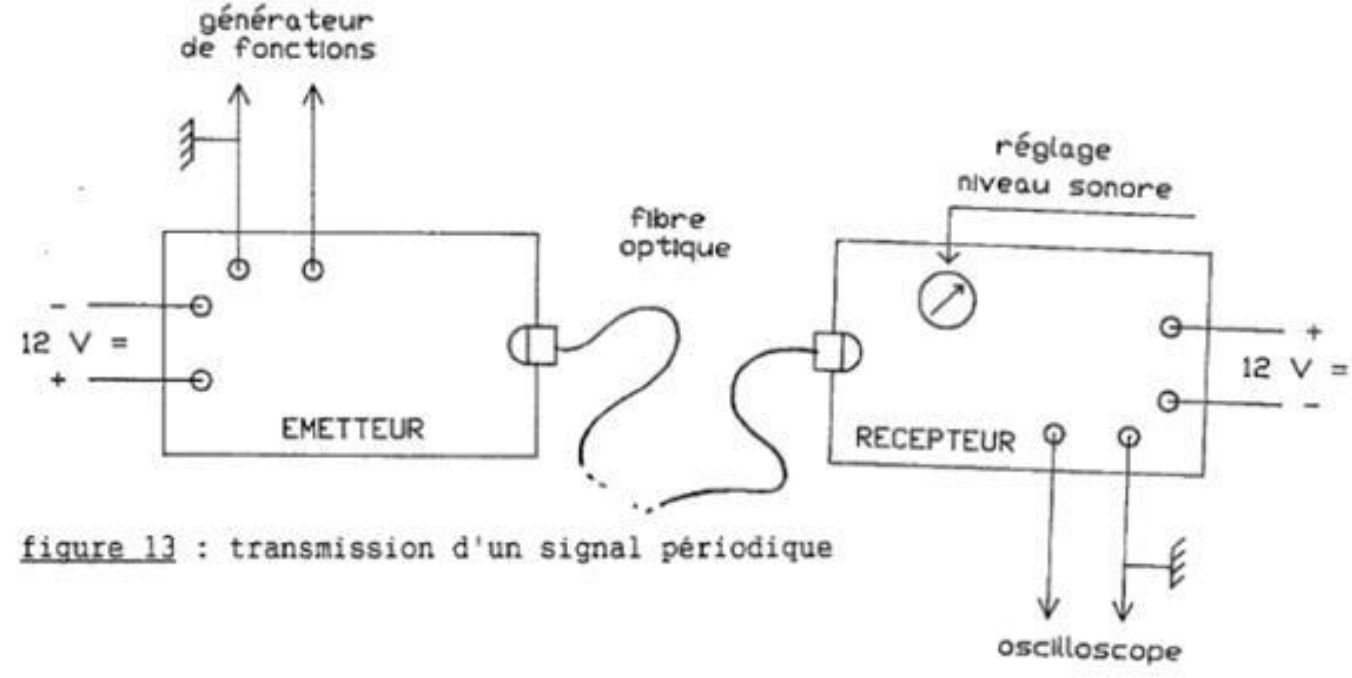
\includegraphics[width=0.85\textwidth]{images/montage04.PNG}
    \caption{Montage de l'expérience n\textdegree8}
    \label{fig:montage04}
\end{figure}

\begin{center}
    Signal sinusoïdal $\rightarrow$ Emetteur $\rightarrow$ Signal Infrarouge $\rightarrow$ Récepteur $\rightarrow$ Oscilloscope 
\end{center}

Observations:
\begin{itemize}
    \item On peut observer que le signal sinusoïdal détecté est aussi périodique mais peut être légèrement déformé. La déformation dépend de la nature du signal, de son amplitude, de sa fréquence et de la valeur de la tension d’alimentation.
    \item Un signal infrarouge modulé par un signal périodique de nature totalement différente passe dans la fibre optique.
    \item En basculant rapidement l’interrupteur, on crée des salves de sinusoïdes.
\end{itemize}

Nous pouvons donc en conclure que le signal électrique, une fois transformé en signal infrarouge par l’émetteur, garde ses caractéristiques de base. Il peut être reçu et, après reconversion en signal électrique, mis à part une légère déformation, sa nature, fréquence et amplitude sont conservées.















\section{Conclusion}





À cause de la quarantaine, nous n'avons pas pu faire les manipulations et nous avons dû imaginer les résultats de chacune des expériences. Heureusement, dans le cas de ce laboratoire, nous avions de explications qui étaient plutôt bonnes et de nombreux schémas pour comprendre comment l'expérience se passait.















\newpage \tableofcontents \listoffigures















\end{document}
